\documentclass[11pt,letterpaper]{article}

% --- Encoding & Language ---
\usepackage[utf8]{inputenc}
\usepackage[T1]{fontenc}
\usepackage[english]{babel}

% --- Page Geometry ---
\usepackage{geometry}
\geometry{top=2.0cm, bottom=2.0cm, left=2.2cm, right=2.2cm}

% --- Typography & Microtypography ---
\usepackage{lmodern}
\usepackage{microtype}
\emergencystretch=1.5em
\tolerance=1000
\raggedbottom

% --- Mathematics & Units ---
\usepackage{amsmath,amssymb}
\usepackage{siunitx}
\sisetup{per-mode=symbol}

% --- Color Palette ---
\usepackage{xcolor}
\definecolor{NavyPrimary}{HTML}{1B365D}
\definecolor{TealAccent}{HTML}{0F766E}
\definecolor{TealBg}{HTML}{F0FDFA}
\definecolor{AmberWarn}{HTML}{B45309}
\definecolor{AmberBg}{HTML}{FFFBEB}
\definecolor{SlateText}{HTML}{334155}
\definecolor{LightPanel}{HTML}{F8FAFC}
\definecolor{BorderGray}{HTML}{CBD5E1}

% --- Tables, Lists & Graphics ---
\usepackage{booktabs}
\usepackage{tabularx}
\usepackage{array}
\usepackage{enumitem}
\usepackage{float}
\usepackage{tikz}
\usetikzlibrary{arrows.meta, positioning, fit, calc, shapes.geometric}

% --- Callout Boxes ---
\usepackage{tcolorbox}
\tcbuselibrary{skins, breakable}

% --- Section Headings ---
\usepackage{titlesec}
\titleformat{\section}
    {\Large\bfseries\color{NavyPrimary}}
    {\thesection.}{0.5em}{}
    [\vspace{-0.4em}\color{NavyPrimary}\rule{\textwidth}{0.8pt}]
\titleformat{\subsection}
    {\large\bfseries\color{TealAccent}}
    {\thesubsection}{0.5em}{}

% --- Headers & Footers ---
\usepackage{fancyhdr}
\setlength{\headheight}{15pt}
\setlength{\footskip}{26pt}
\pagestyle{fancy}
\fancyhf{}
\fancyhead[L]{\small\color{SlateText}COIL Project --- Module 3 Individual Reflection (10\%)}
\fancyhead[R]{\small\color{SlateText}Miguel \'Angel Rodr\'iguez Payares (161004834)}
\fancyfoot[L]{\small\color{SlateText}Universidad de los Llanos \textbullet\ Sistemas de Comunicaci\'on 2}
\fancyfoot[R]{\small\color{SlateText}Page \thepage}
\renewcommand{\headrulewidth}{0.4pt}
\renewcommand{\footrulewidth}{0.4pt}

% --- Hyperlinks ---
\usepackage{xurl}
\usepackage[
    colorlinks=true,
    linkcolor=NavyPrimary,
    citecolor=NavyPrimary,
    urlcolor=TealAccent,
    pdftitle={COIL Project - Module 3 Individual Reflection},
    pdfauthor={Miguel Angel Rodriguez Payares}
]{hyperref}

\begin{document}

% --- Executive Academic Title Banner ---
\thispagestyle{plain}
\begin{tcolorbox}[
    enhanced,
    colback=NavyPrimary,
    colframe=NavyPrimary,
    arc=4pt,
    left=12pt,
    right=12pt,
    top=9pt,
    bottom=9pt
]
{\color{white}\large\bfseries COIL International Exchange --- Module 3 Individual Reflection (10\%)}\\[2pt]
{\color{BorderGray}\small Lessons Learned from COIL: Critical Incident Analysis and Academic Growth}\\[6pt]
{\color{white}\footnotesize
\textbf{Student:} Miguel \'Angel Rodr\'iguez Payares (ID: 161004834) \quad|\quad \textbf{Program:} Electronic Engineering (10th Semester)\\
\textbf{Institutions:} Universidad de los Llanos (Colombia) \& Seneca Polytechnic (Canada) \quad|\quad \textbf{Course:} Sistemas de Comunicaci\'on 2\\
\textbf{Team:} Group 2 \quad|\quad \textbf{Submission Window:} November 16 -- November 22, 2026
}
\end{tcolorbox}

\vspace{0.1cm}

\begin{table}[H]
\centering
\small
\begin{tabularx}{\textwidth}{@{} >{\bfseries}l >{\raggedright\arraybackslash}X >{\bfseries}l @{}}
\toprule
\textbf{Module Component} & \textbf{Included Deliverable} & \textbf{Weight} \\
\midrule
Part 1: Critical Incident Analysis & Option A (300-word formal essay) + Option B (1-minute video script, 146~words) & 5\% \\
Part 2: Academic Growth \& Development & Detailed responses to Question~1 (2.5\%) and Question~2 (2.5\%) & 5\% \\
\bottomrule
\end{tabularx}
\end{table}

\section{Part 1: Critical Incident Analysis (5\%)}

This section addresses Part~1 of Module~3 using both rubric formats on the exact same Group~2 factual narrative: a 300-word written summary (Option~A) and a synchronized one-minute oral presentation script (Option~B).

\subsection{Option A: Written Critical Incident Summary (300 Words)}

\begin{tcolorbox}[
    enhanced,
    breakable,
    colback=LightPanel,
    colframe=NavyPrimary,
    boxrule=0.8pt,
    arc=4pt,
    left=10pt,
    right=10pt,
    top=8pt,
    bottom=8pt,
    title={\textbf{Critical Incident Written Analysis --- Miguel \'Angel Rodr\'iguez Payares}},
    fonttitle=\small\bfseries,
    coltitle=white,
    colbacktitle=NavyPrimary
]
During our COIL Group~2 collaboration between Universidad de los Llanos in Colombia and Seneca Polytechnic in Canada, the primary critical incident emerged at the very outset of the project. Although the technical assignment required an interconnected Software-Defined Wide Area Network linking servers and student clients across both institutions, we experienced a complete absence of contact from our assigned Seneca Polytechnic counterparts from the beginning of the exchange. Neither initial outreach messages nor coordination attempts through the shared course channels produced a reply, leaving our bilateral team without active Canadian participation.

This communication breakdown created a severe operational obstacle. According to the Module~2 guidelines, Seneca students were responsible for configuring the authoritative DNS server inside the overlay network and deploying their institutional cultural intranet, while both universities were expected to negotiate and sign a Group Contract. Without partner engagement, our UniLlanos sub-team faced the risk of being unable to validate cross-institutional domain resolution, end-to-end TLS encryption, or live Wireshark traffic capture.

To prevent project failure, my UniLlanos teammate, Luis Alejandro Le\'on Vel\'asquez, and I documented the lack of response and established an internal contingency plan. I assumed end-to-end architecture for the ZeroTier SD-WAN overlay, the RFC-compliant authoritative DNS service, our private Root Certificate Authority, the dual-protocol HTTPS server, and a secondary gateway node simulating the Seneca endpoint. I also researched Canadian landmarks, traditions, and gastronomy to build the Seneca cultural intranet respectfully, while Alejandro administered the ZeroTier Central network and verified domain navigation from an external physical client node across the Americas.

This experience taught me that international engineering projects often fail not over code or protocols, but due to early coordination gaps and academic calendar mismatches. Proactive contingency planning, clear documentation, and willingness to absorb critical dependencies transformed an initial deadlock into a fully verified, cross-cultural technical delivery.
\end{tcolorbox}

\noindent\textit{Verified length: 300~words across four cohesive paragraphs covering context, impact, technical resolution, and intercultural reflection.}

\subsection{Option B: One-Minute Video Presentation Script}

The following monologue condenses the critical incident narrative into a clear 60-second delivery format (146~spoken words at a natural speaking cadence of 145--150~words per minute). Table~\ref{tab:video_script_timing} provides scene timing cues for recording or voiceover synchronization, followed by the continuous script block.

\begin{table}[H]
\centering
\caption{Timed Delivery Breakdown for the One-Minute Critical Incident Video (Option~B).}
\label{tab:video_script_timing}
\small
\begin{tabularx}{\textwidth}{@{} >{\bfseries}l >{\bfseries}l >{\raggedright\arraybackslash}X @{}}
\toprule
\textbf{Time Window} & \textbf{Rubric Beat} & \textbf{Visual / Screen Cue} \\
\midrule
0:00 -- 0:14 & Context & Title card or webcam introduction showing COIL Group~2 header and UniLlanos affiliation. \\
0:14 -- 0:28 & Challenge \& Impact & Brief view of Module~2 topology highlighting Seneca's planned DNS and intranet dependencies. \\
0:28 -- 0:47 & Technical Resolution & Show ZeroTier Central (\texttt{abfd31bd47affa39}), dual HTTPS portal, and \texttt{https://www.coil-group2.com/seneca/}. \\
0:47 -- 1:00 & Lesson Learned & Closing slide or direct camera view summarizing proactive ownership and cross-cultural learning. \\
\bottomrule
\end{tabularx}
\end{table}

\begin{tcolorbox}[
    enhanced,
    colback=TealBg,
    colframe=TealAccent,
    boxrule=0.8pt,
    arc=4pt,
    left=10pt,
    right=10pt,
    top=8pt,
    bottom=8pt,
    title={\textbf{Continuous Oral Script (146 Spoken Words --- Approx. 60 Seconds)}},
    fonttitle=\small\bfseries,
    coltitle=white,
    colbacktitle=TealAccent
]
``Hello everyone, my name is Miguel \'Angel Rodr\'iguez Payares, a tenth-semester Electronic Engineering student at Universidad de los Llanos. During our Group~2 COIL exchange with Seneca Polytechnic, we faced a critical incident right from the start: complete silence from our assigned Canadian partners.

Because Seneca was originally expected to host the DNS service and their cultural intranet, and both sides needed to sign a Group Contract, this lack of communication threatened our ability to demonstrate domain-based HTTPS connectivity.

Instead of stalling, my teammate Luis Alejandro Le\'on and I agreed on a contingency plan. I deployed the ZeroTier SD-WAN, the authoritative DNS server, a custom Root CA, both cultural intranets, and a simulated Seneca gateway, while Alejandro managed ZeroTier Central and external client verification.

This taught me that resilient engineering depends on early verification, clear documentation, and proactive ownership whenever international coordination breaks down. Thank you.''
\end{tcolorbox}

Figure~\ref{fig:contingency_workflow} summarizes how this critical incident shifted the project from an initial bilateral deadlock to a validated full-stack implementation.

\begin{figure}[H]
\centering
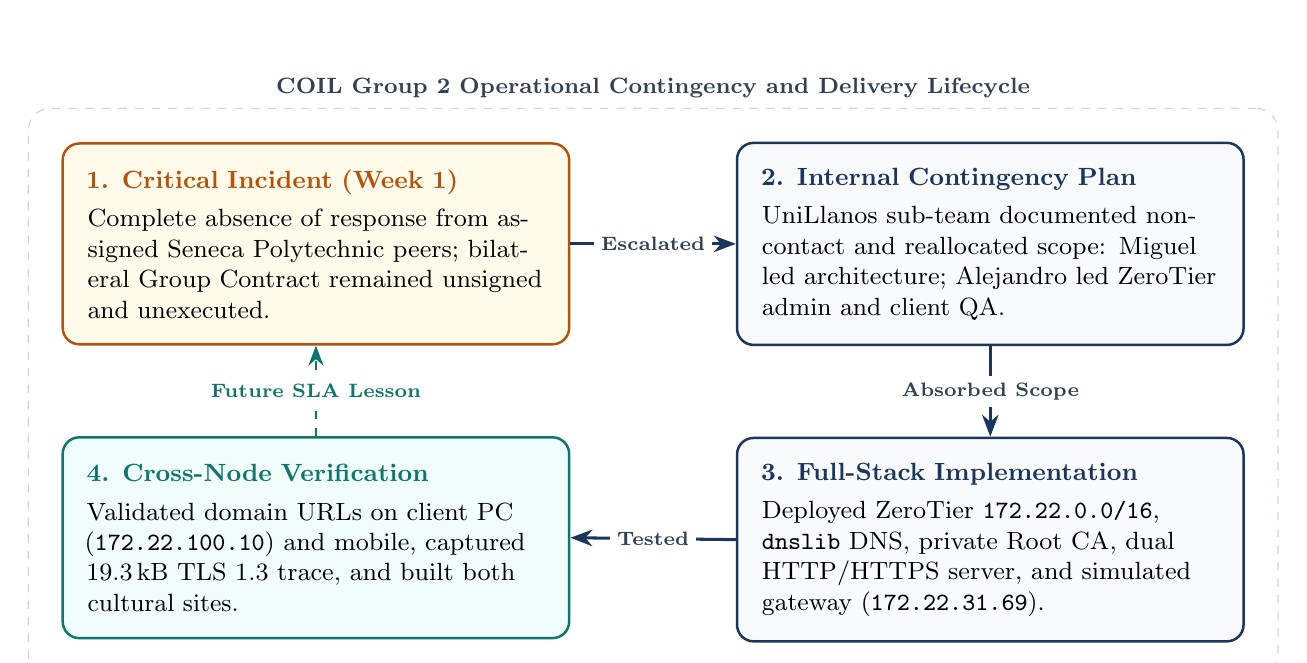
\begin{tikzpicture}[
    node distance=1.15cm and 2.1cm,
    stage/.style={
        rectangle,
        rounded corners=6pt,
        draw=NavyPrimary,
        fill=LightPanel,
        line width=0.9pt,
        text width=5.8cm,
        align=left,
        inner sep=9pt,
        minimum height=2.55cm,
        font=\small
    },
    incident/.style={
        stage,
        draw=AmberWarn,
        fill=AmberBg
    },
    verified/.style={
        stage,
        draw=TealAccent,
        fill=TealBg
    },
    flow/.style={
        ->,
        >=Stealth,
        line width=1.1pt,
        color=NavyPrimary
    },
    feedback/.style={
        ->,
        >=Stealth,
        dashed,
        line width=0.95pt,
        color=TealAccent
    },
    edgelabel/.style={
        font=\scriptsize\bfseries,
        fill=white,
        inner sep=2.5pt,
        text=SlateText
    }
]

\node[incident] (stage1) {
    \textbf{\color{AmberWarn}1. Critical Incident (Week 1)}\\[3pt]
    Complete absence of response from assigned Seneca Polytechnic peers; bilateral Group Contract remained unsigned and unexecuted.
};

\node[stage, right=of stage1] (stage2) {
    \textbf{\color{NavyPrimary}2. Internal Contingency Plan}\\[3pt]
    UniLlanos sub-team documented non-contact and reallocated scope: Miguel led architecture; Alejandro led ZeroTier admin and client QA.
};

\node[stage, below=of stage2] (stage3) {
    \textbf{\color{NavyPrimary}3. Full-Stack Implementation}\\[3pt]
    Deployed ZeroTier \texttt{172.22.0.0/16}, \texttt{dnslib} DNS, private Root CA, dual HTTP/HTTPS server, and simulated gateway (\texttt{172.22.31.69}).
};

\node[verified, below=of stage1] (stage4) {
    \textbf{\color{TealAccent}4. Cross-Node Verification}\\[3pt]
    Validated domain URLs on client PC (\texttt{172.22.100.10}) and mobile, captured \SI{19.3}{\kilo\byte} TLS~1.3 trace, and built both cultural sites.
};

\node[draw=BorderGray, dashed, rounded corners=8pt, inner sep=12pt, fit=(stage1) (stage2) (stage3) (stage4), label={[font=\footnotesize\bfseries\color{SlateText}]above:{COIL Group 2 Operational Contingency and Delivery Lifecycle}}] (container) {};

\coordinate (mid_top) at ($(stage1.east)!0.5!(stage2.west)$);
\coordinate (mid_right) at ($(stage2.south)!0.5!(stage3.north)$);
\coordinate (mid_bot) at ($(stage3.west)!0.5!(stage4.east)$);
\coordinate (mid_left) at ($(stage4.north)!0.5!(stage1.south)$);

\draw[flow] (stage1.east) -- (stage2.west);
\node[edgelabel] at (mid_top) {Escalated};

\draw[flow] (stage2.south) -- (stage3.north);
\node[edgelabel] at (mid_right) {Absorbed Scope};

\draw[flow] (stage3.west) -- (stage4.east);
\node[edgelabel] at (mid_bot) {Tested};

\draw[feedback] (stage4.north) -- (stage1.south);
\node[edgelabel, text=TealAccent] at (mid_left) {Future SLA Lesson};

\end{tikzpicture}
\caption{Critical incident escalation, internal role reallocation, and full-stack contingency workflow executed by the Universidad de los Llanos sub-team.}
\label{fig:contingency_workflow}
\end{figure}


\section{Part 2: Academic Growth and Development (5\%)}

\subsection{Question 1: Project Responsibilities and New Technical Skills (2.5\%)}

\begin{tcolorbox}[
    colback=LightPanel,
    colframe=BorderGray,
    boxrule=0.7pt,
    arc=3pt,
    left=9pt,
    right=9pt,
    top=6pt,
    bottom=6pt
]
\textbf{Prompt:} \textit{``Through the course of the COIL project and your participation in it, explain which part(s) of the project you were responsible for, and what new technical skills you have developed while completing your portion of the project.''}
\end{tcolorbox}

Because our assigned Seneca Polytechnic counterparts never established contact, the technical workload of COIL Group~2 had to be absorbed entirely by our two-person team at Universidad de los Llanos. Within our internal division of responsibilities, my partner Luis Alejandro Le\'on Vel\'asquez owned ZeroTier Central network administration and external physical client testing (\texttt{f6fcd4ce4d} at \texttt{172.22.100.10/16}), while I assumed architectural and implementation ownership for the core networking, cryptographic, web application, packet-inspection, and documentation layers of the project.

Specifically, I was responsible for five integrated subsystems. First, I designed and operated the host overlay topology on ZeroTier Network ID \texttt{abfd31bd47affa39} (\texttt{172.22.0.0/16}), deploying both the primary server node (\texttt{aed30a4fdd}, \texttt{172.22.201.2/16}) and a secondary node (\texttt{1c84e39095}, \texttt{172.22.31.69/16}) that simulated the missing Seneca gateway so cross-node verification remained authentic. Second, I programmed the multi-threaded dual-protocol web server (\texttt{server\_https.py}) listening on ports 80 and 443, and developed the responsive HTML5/CSS3 gateway portal alongside both the UniLlanos and Seneca cultural intranets. Third, to fulfill the strict HTTPS requirement and achieve the bonus trust criteria, I designed an internal Public Key Infrastructure (\texttt{openssl.cnf}), generated a 2048-bit RSA Root Certificate Authority (\texttt{COIL Group 2 Root CA}), and issued Subject Alternative Name (SAN) leaf certificates covering every domain and virtual IP. Fourth, I absorbed Seneca's originally assigned DNS scope by building an RFC-compliant authoritative and forwarding DNS server (\texttt{dns\_server.py}) using \texttt{dnslib} on UDP port~53, complemented by automated PowerShell host-setup and batch launch scripts. Fifth, I captured live SD-WAN traffic in Wireshark (\texttt{coil\_sdwan\_https\_traffic.pcapng}, \SI{19.3}{\kilo\byte}) and authored the formal Module~2 English technical report, four step-by-step manuals, and demonstration scripts.

Completing these subsystems forced me to move beyond textbook theory and develop several practical systems-engineering skills through real troubleshooting:

\begin{itemize}[leftmargin=1.4em, itemsep=4pt]
    \item \textbf{RFC-Compliant DNS Engineering and Mobile Diagnostics:} While testing smartphone access over ZeroTier (\texttt{172.22.201.50}), Android's \texttt{netd} resolver failed with \texttt{FORMERR} because initial responses lacked authoritative \texttt{SOA} records on \texttt{NODATA} replies for IPv6 (\texttt{AAAA}) and \texttt{HTTPS} (Type~65) queries. I also diagnosed a ZeroTier Search Domain suffix loop (\texttt{www.coil-group2.com.coil-group2.com}) triggering \texttt{DNS\_PROBE\_STARTED}, and cleared a Windows \texttt{SharedAccess} (ICS) UDP~53 port conflict.
    \item \textbf{Concurrent TLS Socket Handling:} Standard synchronous SSL wrapping blocks the server accept loop when clients probe and stall, and calling \texttt{shutdown(SHUT\_WR)} on wrapped Windows TLS sockets can emit TCP \texttt{RST} frames that trigger \texttt{ERR\_CONNECTION\_CLOSED}. Implementing \texttt{NonBlockingSSLThreadingServer} with worker-thread handshakes and bounded timeouts taught me production-safe TLS concurrency.
    \item \textbf{Custom X.509 v3 PKI and OS Trust Stores:} Configuring \texttt{basicConstraints}, \texttt{authorityKeyIdentifier}, and SAN entries in OpenSSL, then automating Root CA installation into Windows (\texttt{Cert:\textbackslash LocalMachine\textbackslash Root}) and Android, gave me hands-on mastery of browser trust chains.
    \item \textbf{Overlay MTU Tuning and Deep Packet Inspection:} Tuning ZeroTier's virtual interface MTU to \SI{1300}{bytes} prevented cellular fragmentation, adjusting Windows firewall interface profiles from \texttt{Public} to \texttt{Private} unblocked inbound routing, and applying Wireshark display filters (\texttt{ip.addr == 172.22.31.69 and tcp.port == 443}) sharpened my ability to audit TCP 3-way handshakes, TLS~1.3 1-RTT exchanges (\texttt{X25519}, \texttt{TLS\_AES\_256\_GCM\_SHA384}), and orderly \texttt{FIN/ACK} teardowns.
\end{itemize}

Table~\ref{tab:responsibilities_skills} maps each project responsibility directly to its concrete deliverable and the engineering competencies acquired.

\begin{table}[H]
\centering
\caption{Summary of Miguel \'Angel Rodr\'iguez Payares's Technical Responsibilities and Acquired Skills.}
\label{tab:responsibilities_skills}
\small
\begin{tabularx}{\textwidth}{@{} >{\bfseries\raggedright\arraybackslash}p{2.9cm} >{\raggedright\arraybackslash}p{5.55cm} >{\raggedright\arraybackslash}X @{}}
\toprule
\textbf{Subsystem} & \textbf{Concrete Deliverables} & \textbf{New Technical Skills Developed} \\
\midrule
SD-WAN Overlay \& Firewalling & ZeroTier \texttt{abfd31bd47affa39} host (\texttt{172.22.201.2}) and simulated gateway (\texttt{172.22.31.69}) & Virtual interface MTU tuning (\SI{1300}{bytes}), Windows \texttt{Private} profile routing, and cross-node ICMP diagnostics. \\
\addlinespace[4pt]
Authoritative DNS Service & \path{dns_server.py} (\texttt{dnslib}), \path{setup_hosts.ps1}, and \path{iniciar_pagina.bat} & RFC~1035/2308 \texttt{SOA} \texttt{NODATA} handling for \texttt{AAAA}/Type~65, upstream forwarding, and UDP~53 port conflict recovery. \\
\addlinespace[4pt]
Custom PKI \& TLS~1.3 & \texttt{openssl.cnf}, \path{COIL_Group2_Root_CA.crt}, SAN cert, and \path{install_root_ca.ps1} & X.509 v3 Root CA chaining, multi-SAN signing, and Windows/Android trust-store deployment (bonus compliance). \\
\addlinespace[4pt]
Multi-Tenant Web Server & \path{server_https.py}, gateway portal, \texttt{/unillanos/}, and \texttt{/seneca/} frontends & Thread-safe non-blocking TLS wrapping, dual HTTP/HTTPS sockets, host/path routing, and responsive HTML5/CSS3 design. \\
\addlinespace[4pt]
Traffic Audit \& Documentation & \texttt{coil\_\-sdwan\_\-https\_\-traffic.pcapng}, 4~Wireshark screenshots, report, and scripts & Boolean packet filtering, TLS~1.3 cipher/SNI dissection, TCP state-machine verification, and formal English technical writing. \\
\bottomrule
\end{tabularx}
\end{table}

\subsection{Question 2: Group Contract Comparison and Reflection (2.5\%)}

\begin{tcolorbox}[
    colback=LightPanel,
    colframe=BorderGray,
    boxrule=0.7pt,
    arc=3pt,
    left=9pt,
    right=9pt,
    top=6pt,
    bottom=6pt
]
\textbf{Prompt:} \textit{``Compare what you have completed in the project to the original Group Contract that was signed. Was the group contract followed? Please elaborate and reflect on why the contract was or wasn't followed.''}
\end{tcolorbox}

To answer honestly and directly: \textbf{no, the original bilateral Group Contract was not followed, because it was never formally signed or put into effect with our Seneca Polytechnic counterparts.} From the initial launch of the COIL exchange, our assigned Canadian teammates never responded to outreach messages or joined any planning touchpoints. Consequently, a shared cross-institutional agreement governing meeting schedules, communication response windows, and joint deliverables could not be negotiated or signed.

Faced with complete silence from the partner side, Luis Alejandro Le\'on Vel\'asquez and I faced a clear risk of leaving critical dependencies---specifically the authoritative DNS server and Seneca's cultural intranet---unbuilt. Rather than allowing an unexecuted contract to block our progress on Module~2 (which carries 80\% of the project grade), we established an informal internal working agreement within Universidad de los Llanos. Under this contingency pact, we preserved 100\% of the technical objectives defined in the course guide by reallocating Seneca's unfulfilled responsibilities to ourselves and documenting every step transparently.

Table~\ref{tab:contract_comparison} contrasts the original bilateral project governance model envisioned by the COIL activity against what our UniLlanos sub-team actually executed.

\begin{table}[H]
\centering
\caption{Comparison Between the Planned Bilateral Group Contract Model and Actual Execution.}
\label{tab:contract_comparison}
\small
\begin{tabularx}{\textwidth}{@{} >{\bfseries\raggedright\arraybackslash}p{2.7cm} >{\raggedright\arraybackslash}X >{\raggedright\arraybackslash}X >{\raggedright\arraybackslash}p{2.7cm} @{}}
\toprule
\textbf{Project Element} & \textbf{Planned Bilateral Contract} & \textbf{Actual Execution (UniLlanos)} & \textbf{Outcome} \\
\midrule
Signed Group Contract & Jointly negotiated rules, roles, and meeting cadence across both schools & Never signed due to zero Seneca contact; replaced by internal UniLlanos pact & Not Followed (Contingency Used) \\
\addlinespace[4pt]
ZeroTier SD-WAN Mesh & At least one PC per student across Seneca and UniLlanos & Miguel host (\texttt{172.22.201.2}), Alejandro client (\texttt{172.22.100.10}), simulated gateway (\texttt{172.22.31.69}), mobile & Completed Internally \\
\addlinespace[4pt]
Authoritative DNS Server & Configured and operated by Seneca students & Designed and deployed in Python (\texttt{dnslib}) by Miguel on UDP~53 & Reallocated \& Completed \\
\addlinespace[4pt]
Cultural Intranet Sites & UniLlanos builds Colombian site; Seneca builds Canadian site & UniLlanos built both \texttt{/unillanos/} and \texttt{/seneca/} portals with authentic research & Reallocated \& Completed \\
\addlinespace[4pt]
HTTPS, PKI \& Bonus Trust & Self-signed TLS required; trusted Root CA optional bonus & Full OpenSSL Root CA + SAN certs installed in OS trust stores (zero warnings) & Completed + Bonus Met \\
\addlinespace[4pt]
Wireshark, Report \& Videos & Joint English technical report and individual member videos & Full \SI{19.3}{\kilo\byte} PCAP, 4~packet figures, 4~manuals, and UniLlanos individual demos & Completed by UniLlanos \\
\bottomrule
\end{tabularx}
\end{table}

Reflecting critically on \textit{why} the Group Contract was never signed or followed reveals three structural root causes common to international virtual exchanges:

\begin{enumerate}[leftmargin=1.4em, itemsep=4pt]
    \item \textbf{Absence of a Verified Week~1 Synchronous Kickoff:} Without a mandatory live video orientation where both sides confirm active course enrollment, verify email or messaging handles, and co-sign the contract in real time, asynchronous outreach fails silently. Once initial momentum is lost during the first week, re-engaging unresponsive remote members becomes exceedingly difficult.
    \item \textbf{Institutional and Academic Calendar Asymmetry:} Partner cohorts across Colombia and Canada operate under different semester timelines, add/drop windows, workload peaks, and grading weights. If students from one institution drop the course, change sections, or deprioritize an unaligned assignment before team formation stabilizes, the bilateral contract collapses before technical work even begins.
    \item \textbf{Lack of an Automated Early-Escalation Clause:} The standard COIL workflow assumed bilateral participation would materialize organically, without specifying a strict 72-hour response Service Level Agreement (SLA) or an automatic instructor-mediated reassignment mechanism when a partner team goes silent.
\end{enumerate}

Ultimately, while the formal cross-institutional Group Contract could not be followed, the discipline of honoring its underlying technical and ethical standards led us to a stronger outcome. Within UniLlanos, Alejandro and I maintained clear accountability, met our technical milestones ahead of deadlines, and never lowered the engineering bar just because a partner was absent. In future international collaborations, I will insist on three safeguards from day one: a synchronous verification call in Week~1, explicit response-time SLAs with an instructor escalation trigger, and decoupled system interfaces so that a sub-team can always test and deliver reliably even when external dependencies fail.


\end{document}
